\documentclass[10pt]{article}
\usepackage[utf8]{inputenc}


\usepackage{graphicx}
\usepackage{wrapfig}

\title{IF793 - PROJETO IMPLEMENTAÇÃO DE JOGOS 2D}
\author{Thaís Vasconcelos Couto}
\date{03 de novembro de 2019}

\usepackage{natbib}
\usepackage{graphicx}

\begin{document}

\maketitle

\section{Introdução}
\paragraph{} A disciplina Projeto Implementação de Jogos 2D é uma cadeira eletiva oferecida aos alunos do CIn, graduandos em Ciência da Computação, desde o ano de 2000, sendo a primeira do gênero no Brasil. Durante o semestre, os alunos devem criar um jogo 2D em grupos. Existe auxílio desde a criação da ideia do jogo, até a seu desenvolvimento e implementação. Os alunos desenvolvem seus jogos de acordo com os conceitos novos apresentados em cada aula. Desse modo, a apresentação do novo jogo resultará na nota de cada aluno no final do período. 


\begin{figure}[h!]
\centering
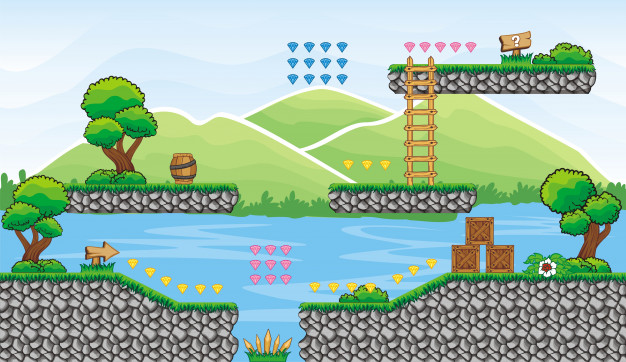
\includegraphics[width = 7cm]{jogo2d.jpg}
\caption{Exemplo de jogo 2D}
\end{figure}

\paragraph{}Alguns dos materiais bibliográficos utilizados durante a disciplina são:
\begin{itemize}
    \item\cite{salen2004rules} Game Architecture and Design with Cdrom
    \item\cite{kostertheory} Rules of play: Game design fundamentals
    \item\cite{rollings1999game} Theory of Fun for Game Design
 \end{itemize}
\paragraph{}


\section{Relevância}
\paragraph{} Atualmente, os jogos estão crescendo cada vez mais no mercado de informática. Por isso, essa disciplina é extremamente importante, ja que oferece uma boa oportunidade aos alunos de aprenderem novos conceitos sobre uma área muito importante não só no mercado pernambucano, que por sinal, vem investindo muito na área de jogos, mas também no mercado mundial. 

\section{Relação com outras disciplinas}
\paragraph{} Os pré-requisitos necessários para cursar essa disciplina são outras 3 cadeiras (listadas abaixo), as quais lidam com aprendizagem de máquinas, gráficos, in-terfaces, elementos de realidade virtual, entre outros conhecimentos necessários para a criação de um jogo.
\begin{itemize}
    \item IF680 - Processamento Gráfico
    \item IF684 - Sistemas Inteligentes
    \item IF687 - Introdução à multimídia
 \end{itemize}
\paragraph{} 

\bibliographystyle{plain}
\bibliography{tvc}
\end{document}
